\chapter{The $\alpha$-shapes approach to compute the boundaries in target phase space}\label{chap:boundaries_alpha}
The $\alpha$-shape method which is widely used for reconstruction an unknown surface from a set of data points.
We develop a technique based on $\alpha$-shape to obtain an approximation of the boundaries of the set of points obtained from the triangulation refinement, \cite{guo1997surface}.
The aim is to give a criterion to determine the value of the parameter $\alpha$ that gives the better approximation of the boundaries.
The results are given in Section \ref{sec:Tir_alpha} for two different kind of Total Internal reflection (TIR) collimator.
\section{The $\alpha$-shapes approach}
Given a finite set $V$ of points $\alpha$-shapes are geometrical objects that give us an approximation of the "shape"\footnote{It will become clear through this chapter what we intend with the word \textit{shape}.} formed by the points in the set.\\ \indent
Before giving a formal definition, we explain an intuitive and nice interpretation of $\alpha$-shapes. 
We can think to a mass of a stracciatella\footnote{Stracciatella ice cream is made with milk-based ice-cream and fine peaces of chocolate, \cite{Wiki3}.} ice-cream. If we desire to know the shape formed by the chocolate pieces, we can start eat the ice cream using a spoon with a spherical shape trying to do not remove any piece of chocolate. 
We will obtain a shape formed by arcs and points, see Figure \ref{fig:shape2d} for the two-dimensional case.
\begin{figure}[htbp]\label{fig:shape2d}
\begin{center}
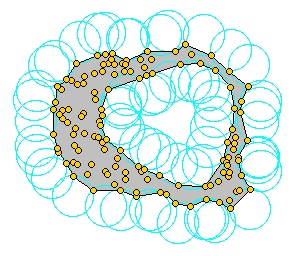
\includegraphics[width=7cm]{shape.jpg}
\label{fig:shape}
\caption{Construction of $\alpha$-shape given a set of points in $\mathbb{R}^2$}
\label{fig:shape2d}
\end{center}
\end{figure}
Straightening the arcs to line segments we obtain broken lines which constitute the boundaries the so-called $\alpha$-shape of $V$. In the ice-cream example, the chocolates peaces are the points of the point set and, the parameter $\alpha$ determines the radius of the carving spoon (the spherical spoon in two-dimension is simply a circle). A very small spoon will allow us to eat the entire ice cream without eating any piece of chocolate, while with a huge spoon we are not able to eat any part of the ice cream because we will always take away at least one chocolate peace.\\ \indent 
The previous example might give a better understanding of the definition of $\alpha$-shape first given by Edelsbrunner, Kirkpatrick and Seidel in 1983, \cite{edelsbrunner1983shape}. In their paper they describe the $\alpha$-shape has a generalization of the convex hull of a finite set of point in the plane. Let be $\alpha$ a not negative number $0\leq\alpha<\infty$. 
If $\alpha$ is equal to $0$ the shape degenerates to the point set $V$. On the other hand, when $\alpha\rightarrow\infty$ the $\alpha$-shape is simply the convex hull. Finally, if $0<\alpha<\infty$ the $\alpha$-shape is a polytope of the point set, \cite{edelsbrunner1994three}. The $\alpha$-shapes are closely related to Delaunay triangulation of $V$,\cite{mucke1993shapes}.\\ \indent
Given a set $V$ of not all aligned points, let us consider the set $E$ of all the straight line segments whose endpoints are in $V$. 
A triangulation $T$ of $V$ is the maximum subset of $E$ such that all the line segments of $T$ intersect only at their endpoints, \cite{lloyd1977triangulations}. \\ \indent 
Delaunay triangulation can be seen as the dual of Voronoi diagram, \cite{fortune1992voronoi}.\\\indent
We give here the definition Voronoi diagram only in two dimensions, (see \cite{brown1979voronoi} for the general case).
In every finite set of point $V = \{v_1, \cdots, v_n\}\subset \mathbb{R}^2$ and for \textit{almost}\footnote{It is needed to specify the word \textit{almost} because some points can have the same distance with two or more points of $V$.} every point $x\in \mathbb{R}^2$, there is a point which is the closest point to $x$. The Voronoi cell of a point $v_\variabile{i}\in V$ contains all points in $\mathbb{R}^2$ which are closer to $v_{\variabile{i}}$, see Figure {fig:Voronoi}. 
The Voronoi diagram is the set of all Voronoi cells, \cite{cazals2005conformal}.
A formal definition of the Voronoi diagram is given in the following.
\begin{defn}
Let $X$ be a metric space with a distance $\textrm{d}$ and $V=\{v_1,\cdots,v_n\}$ a set of point in $X$. The Voronoi cell $V_\variabile{i}$ associated with the point $v_\variabile{i}$ with $v_{\variabile{i}}\in\{1,\cdots,n\}$ is defined as:
\begin{equation}
V_\variabile{i}=\{x\in X\; | \;\textrm{d}(x,v_\variabile{i})\leq \textrm{d}(x,v_\variabile{j}) \quad \forall \variabile{j}\neq \variabile{i} \}\,,
\end{equation}
The Voronoi diagram is defined as the union $U = \bigcup_{\variabile{i}=1}^n V_\variabile{i}$ where $V_{\variabile{i}}\cap V_{\variabile{j}}= \emptyset$ for $\variabile{i}\neq\variabile{j}$.
\end{defn}
Figure \ref{fig:Voronoi}
\begin{figure}[h]\label{fig:Voronoi}
\begin{center}
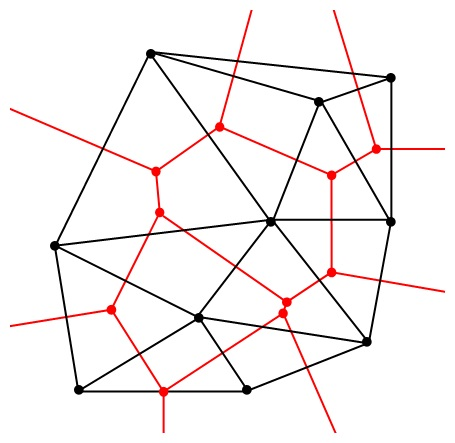
\includegraphics[width=7cm]{Delaunay_Voronoi.jpg}
\caption{The Delaunay triangulation in black is the dual of the Voronoi diagram in red, \cite{Wiki4}.}
\label{fig:Voronoi}
\end{center}
\end{figure}
The Delaunay triangulation of the points set $V$ has the property (also called Delaunay property) that the circle circumscribed by any triangle of $T$ does not contain any point of $V$. A very common used algorithm to construct such triangulation is explained in the following. 
A Delaunay triangulation is constructed by modifying a general triangulation $T$ such that every point satisfies the Delaunay property. 
Therefore, every triangle (or tetrahedron in three dimensions) that does not satisfy such property is flipped such that the new edge is part of the triangulation. 
More precisely, given an arbitrary triangulation $T$ in two-dimension, for each edge $\bar{ab}$ in $T$ which is not on the boundary of the convex hull the two triangles 
$\Delta_{abc}$ and $\Delta_{abd}$ with the common edge $\bar{ab}$ are found. Then, if either the circumcircle of triangle $\Delta_{abc}$ contains point $d$ or the circumcircle of triangle $\Delta_{abd}$ contains point $c$ the edge $\bar{ab}$ cannot be included in the Delaunay triangulation and, therefore, it is flipped such that the other two possible triangles $\Delta_{acd}$ and $\Delta_{bcd}$ are found. The new edge $\bar{cd}$ satisfy the Delaunay property locally and the triangles are added to the Delaunay triangulation, see Figure \ref{fig:Delaunay}.  
\begin{figure}[h]\label{fig:Delaunay}
\begin{center}
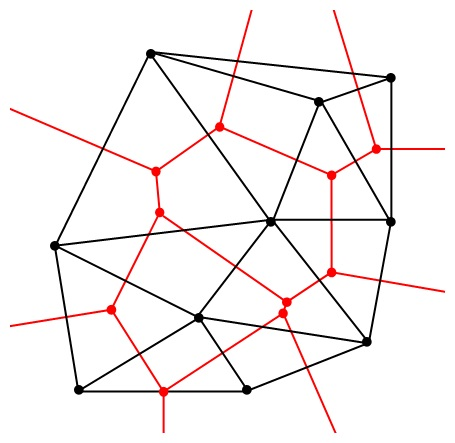
\includegraphics[width=7cm]{Delaunay_Voronoi.jpg}
\label{fig:shape}
\caption{The Delaunay triangulation in black is the dual of the Voronoi diagram in red, \cite{Wiki4}.}
\label{fig:Delaunay}
\end{center}
\end{figure}
\\ \indent Several others algorithm have been developed to construct a Delaunay triangulation, see for example \cite{lee1980two, renka1997algorithm}.
This triangulation is unique for a given set of points $V$. It has the property to have the largest minimum angle among all possible triangulation of a point set $V$, \cite{press2007numerical}. Such triangulation triangulates the convex hull of $V$ and, therefore it does not constitutes a suitable method for reconstruct the surface formed by a point cloud. \\ \indent An important method in surface reconstruction is the $\alpha$-shapes method, \cite{edelsbrunner2010alpha, guo1997surface}. Starting from the Delaunay triangulation $T^\prime$ of a point set $V$, the corresponding $\alpha$-shape of $V$ is formed by the only triangles of $T^\prime$ that satisfy the so-called "$\alpha$-test".
For each triangle we calculate the radius of the circumcircle. If the radius is larger that $\alpha$ the triangle is removed from the shape. The rule of the parameter $\alpha$ is highly significant in this procedure. Hence we have to choose it in such a way to get a better approximation. The choice of the parameter $\alpha$ is closely related to the radius of the circumcircles. A possible strategy is to find the radius of the greater empty circumcircle. Thus $\alpha$ is related to the density of the points. In particular we have:
\begin{equation}
\alpha=C\frac{1}{\Delta}\;,
\end{equation}
with $C$ a constant that can be determined by a simulation and $\Delta$ the density of the point set $V$ defined as:
\begin{equation}
\Delta=\frac{N}{\mbox{surface area}}\; ,
\end{equation}
where $ N $ is the number of points in $V$ and the surface area is the area inside the boundaries of the region formed by the points cloud. Hence $\Delta$ is a constant.
%Let us define a Voronoi diagram in a metric space.

%The simplest case that we can have is the two-dimensional case that is the case where $X=\mathbb{R}^2$.
%The tuple $\mathcal{S}=\{1,\cdots,n\}\subset \mathbb{R}^2$ is now a set of points. The Voronoi diagram of $\mathcal{S}$ is a subsection of $\mathbb{R}^2$ such that every other region around a point $p\in \mathcal{S}$ contains all points that are closer to $p$ than to every point in $\mathcal{S}$. A triangulation of the point set $\mathcal{S}$ is a set of edges $\mathcal{E}$ whose extremes are points of $\mathcal{S}$ such that the faces of each triangle are bounded by three edges and any edge that is not in $\mathcal{E}$ intersects one of the existing edges. The Delaunay triangulation is the dual graph of the Voronoi diagram: it consists of vertices (the points in $\mathcal{S}$) and it has an edge between two vertices if the two corresponding faces share an edge. \\
\indent Even if $\alpha$-shapes are a powerful tool to reconstruct surfaces, some simulations show that there exist surfaces that are not described well by $ \alpha $-shapes. Indeed for some particular surface there exist no value of $\alpha$ that includes all desired triangles and deletes all undesired triangles. For instance, since the parameter $\alpha$ depends on the density of the point cloud, is intuitively clear that using $\alpha$-shapes for a non-uniform points set we won't get a good approximation of the surface. Furthermore, the $\alpha$-shape method doesn't work well when there is a sharp turn or a joint. In this case $\alpha$-shapes often give a "webbed-foot" appearance at such joints since they improperly connect the adjacent surfaces. Hence a generalization of "classical" $\alpha$-shapes is required. In the next section a method to solve the "density problem" for two separated and close objects is described.
In \cite{teichmann1998surface} Teichmann and Capps present "Density-scaled $\alpha$-shapes".
%The first step of this method is to make a triangulation of the point cloud.
%Then the key idea is to compute somehow the point-density of each point and use this to get an approximation of the point density of a triangle. In this way one can reduce the $\alpha$-value in areas where the triangle's point density (see equation \ref{delta_t} for the definition) is higher than average in such a way that is possible to obtain a finer level of detail for areas that have an higher density.
%More precisely, each point $ \textbf{p}\in \mathcal{S} $ has a local point density defined as
%\begin{equation}
%\delta (\textbf{p})= \sum_{\textbf{q}\in \mathcal{S}}\Big( 1-\frac{\textrm{d}(q,p)}{\lambda}\Big) \qquad \forall \textbf{q} \mbox{\;\;such that\;\;} \textrm{d}(\textbf{p},\textbf{q})<\lambda\,,
%\end{equation}
%where $ \lambda $ is the constant radius of the local neighborhood and $\textrm{d}(\textbf{x},\textbf{y})$ is the Euclidean distance.
%When local density is larger than the average, that is when
%\begin{equation}
%\delta (\textbf{p}) >\frac{1}{| \mathcal{S} |}\sum_{\textbf{q}\in \mathcal{S}}\delta (\textbf{q})
%\end{equation}
%we know some properties about the region surrounding $\textbf{p}$.
%For instance, if the point set is uniformly distributed then it is possible to find areas with a high-density in the case where there are two closely separated surfaces.  In point sets of non-uniform distribution, high densities are found when the surface presents a joint discontinuity. The algorithm developed by Teichmann and Capps is structured as follow.
%After computing density information for each point they make a triangulation of the point set. Then they calculate the average density  $\delta(t)$ for each triangle $\Delta_{abc}$ defined as:
%\begin{equation}
%\delta(t)=\frac{\delta(a)+\delta(b)+\delta(c)}{3 \mu}\,,
%\label{delta_t}
%\end{equation}
%where $\mu$ is the global average density of the entire point set $\mathcal{S}$.
%If $\delta(t)$ is greater than $1$ the density of the point cloud is higher. Hence is necessary to define another value of $\alpha$:
%\begin{equation}
%\alpha^{\;\prime} = \frac{\alpha}{\delta(t)^\sigma}
%\end{equation} where $\sigma$ is a value that is adjusted by the user.
%If  $\delta$ is less than $1$ the $\alpha$-value is not modified.
%In this way it is possible to have a finer precision on the shape formed by the point set where the density is higher than the average density. Hence it is possible to distinguish two separated objects with different density.

% We want to determine the boundaries in phase space
% Jorg
% It is useful to understand whether the approximation is correct
\section{Determination of $\alpha$ using \'{e}tendue conservation}
% Explain the idea: use etendue conservation
% Do the example for the two faceted cup
% Explain the TIR collimator
\section{Results for a TIR collimator}
% 
\label{sec:Tir_alpha}

